%------------------------------------------------------------------------------

\chapter{Θεωρία}
\label{chapter3} 

Το κεφάλαιο αυτό θα αναλύσει ότι χρειάζεται να ξέρει ο αναγνώστης για να
κατανοήσει το κεφάλαιο της υλοποίησης. Άρχικα θα περιγράψουμε εκτενέστερα την
διαδικασία που ακολουθείται στο σύστημα RPython για την μεταγλώττιση (π.χ. του
PyPy), έτσι ώστε να ξέρει ο αναγνώστης σε ποιο "χρονικό" σημείο θα λάβει χώρα το
εγχείρημά μας. Έπειτα θα παραθέσουμε με λεπτομέρεια την θεωρία της μεθόδου που
θα υλοποιήσουμε.

%%%%%%%%%%%%%%%%%%%% BALE ALLOU
Η βελτιστοποίηση στο PyPy γίνεται (όπως φαίνεται και στην εικόνα παραπάνω) μετά
το πέρασμα απο τον αναλυτή τύπων. Το project περιλαμβάνει και εφαρμόζει μια
πληθώρα βελτιστοποιήσεων, όπως αυτά που αναφέραμε στο κεφάλαιο 2.\ref{chapter2}

%------------------------------------------------------------------------------

\section{Διαδικασία Μεταγλώττισης στο σύστημα RPython}

\subsection{Επισκόπηση}

Ο σκοπός του συστήματος και του \textit{toolchain} του RPython είναι να
μεταφράσει προγράμματα (κυρίως μεταφραστές) γραμμένα σε RPython με
αποτελεσματικότητα ανεξάρτητα με το ποια πλατοφόρμα είναι το target του. Η
διαδικασία είναι οργανωμένη σε στάδια. Το default target είναι το \textit{C
backend} (παραγωγός κώδικα C) και σε αυτό θα αναφερόμαστε όταν δίνουμε
παραδείγματα.

Το σύστημα στην πραγματικότητα δεν βλέπει ποτέ κανονικό κώδικα Python ή δέντρα,
αλλά ξεκινά με \textit{αντικείμενα κώδικα} (code objects) βασισμένα στις
συναρτήσεις που έχουν δωθεί ως είσοδος. Η \textit{μονάδα} (unit) που βασίζεται το σύστημα επομένως είναι τα function code objects.

\begin{enumerate}

\item Flow Analysis. Εδώ ο αρχικός κώδικας υφίσταται τις βασικές διαδικασίες
συντακικής ανάλυσης, μετατρέπεται αρχικά σε tokens, έπειτα σε μια ενδιάμεση
μορφή (Python bytecode) – όπως σε όλους τους μεταγλωττιστές και τέλος στα
διαγράμματα ροής του PyPy.

\item Annotator subsystem. Εδώ ενεργοποιούνται οι περισσότερο αφαιρετικές
μέθοδοι ερμηνείας του κώδικα.

Περιλαμβάνει annotator και το σύστημα.... TODOOOO

\textbf{RTyper:} Αυτό το σύστημα \textit{υποσημειώνει} τον κώδικα με είδικούς
προσωρινούς τύπους βάσει του context της κάθε μεταβλητής.

\textbf{Exception transformer:} Έπειτα σειρά έχει ο μετατροπέας των
εξαιρέσεων που εισάγει τον απαραίτητο κώδικα για τη
διαχείριση τους.

\textbf{GC Transformer:} Εκτελεί όποιες ενέργειες χρειάζονται για την σωστή
διαχείριση μνήμης.

\item Code Generation. Εδώ τα ήδη μαρκαρισμένα, σημειωμένα, βελτιστοποιημένα
γραφήματα θα μετατραπούν σε κώδικα μηχανής. Εδώ υπάρχουν πολλοί "γεννήτορες"
κώδικα ανάλογα με τις ανάγκες. Ο βασικότερος και ο πιο σημαντικός είναι ο
παραγωγός κώδικα C. Αρχικά, τα γραφήματα θα μετατραπούν σε άλλα αντίστοιχα,
ανάλογα με τον γεννήτορα και έπειτα αυτά θα μετατραπούν σε κώδικα ανάλογα με την
επιλογή (π.χ σε κώδικα C). Τέλος ο κώδικας αυτός θα οδηγηθεί στον μεταφραστή της
εκάστοτε επιλογής (π.χ. \texttt{gcc}).

\end{enumerate}

\begin{figure}[h]
\centering
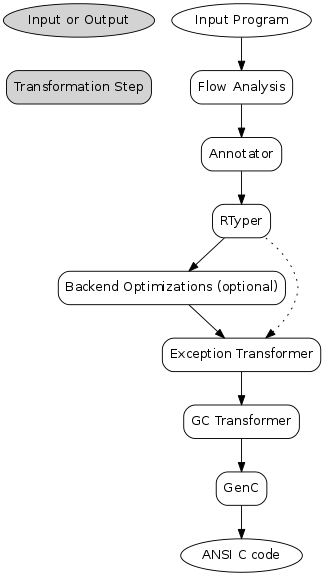
\includegraphics[width=0.5\textwidth]{diagram.png}
\caption{caption test text}
\label{diagram one}
\end{figure}

\subsection{Γραφήματα Ροής}
\subsection{Πέρασμα φδφσδφ}

%------------------------------------------------------------------------------

\section{Θεωρία Μερικής Ανάλυσης Διαφυγής}


\subsection{Απλή Ανάλυση Διαφυγής}

Η μέθοδος που θα αναλύσουμε εκτενώς και θα υλοποιήσουμε λέγεται "Μερική
Ανάλυση Διαφυγής" και είναι φυσικά επέκταση της κανονικής "Ανάλυσης Διαφυγής".
Η τελευταία είναι μια μέθοδος για τον καθορισμό του \textit{δυναμικού πεδίου}
των δεικτών ενός προγράμματος. (Την περιοχή δηλαδή στην οποία είναι ενεργοί
και έγκυροι ή αλλιώς την περιοχή που μπορεί το πρόγραμμα να έχει "πρόσβαση" σε
αυτόν.)\footnote{η απλή ανάλυση διαφυγής είναι ήδη υλοποιημένη στο pypy στο
αρχείο \texttt{escape.py}}

Ένας δείκτης που δημιουργείται από κάποια συνάρτηση μπορεί να
\textit{διαφύγει}σε κάποια άλλη. Τότε το δυναμικό του πεδίο μεγαλώνει. Ένας
δείκτης (ουσιαστικά μια μεταβλητή) λέμε ότι έχει \textit{διαφύγει} όταν μια
συνάρτηση/υπορουτίνα δεσμεύσει μια θέση μνήμης, την αναθέσει σε αυτόν και την
επιστρέψει. Επίσης διαφεύγει αν ανατεθεί σε καθολική (global) μεταβλητή.
Επιπλέον υπάρχουν και άλλοι πιο περίπλοκοι τρόποι διαφυγής όπως στην περίπτωση
functional γλωσσών και tail-call optimization, αλλά δε θα ασχοληθούμε με αυτές
σε αυτή την εργασία.

Με αυτή την μέθοδο καθορίζονται όλα τα μέρη όπου ένας δείκτης μπορεί να
αποθηκευτεί καθώς επίσης και αν η διάρκεια ζωής του δείκτη μπορεί να αποδειχθεί
να περιορίζεται μόνο στην τρέχουσα διαδικασία και/ή το νήμα. (thread)

Η πιο προφανής βελτιστοποίηση με βάση αυτή την ανάλυση είναι η πλήρης εξάλειψη
των δεικτών που δεν διαφεύγουν ή η αντικατάστασή τους με βαθμωτούς μέσα στο
δυναμικό τους πεδίο. Επίσης δυνατή είναι η αντικατάσταση καταχωρήσεων μνήμης
(malloc) στον σωρό (heap) με απλές κατωχηρώσεις στη στοίβα (stack) πράγμα που
κάνει το πρόγραμμα πολύ πιο γρήγορο, και στην περίπτωση γλώσσας με σύστημα
"συλλογής απορριμμάτων" αυτό οδηγεί στο τρέξιμο του συλλέκτη λιγότερες φορές.
Τέλος μπορούμε να έχουμε κάποια οφέλη στα συστήματα συγχρονισμού. Αν ο δείκτης
βρεθεί να μπορεί να προσπελαστεί μόνο από ένα νήμα, τότε μπορούμε να αφαιρέσουμε
τις δομές συγχρονισμού. Εμείς θα ασχοληθούμε μόνο με αντικατάσταση βαθμωτών.


\subsection{Διαφορές και Λεπτομέρειες}


Η "Μερική Ανάλυση Διαφυγής" δουλεύει ομοίως με παραπάνω, αλλά είναι πιο  ισχυρή
με την έννοια ότι λαμβάνει υπόψιν της και τα διάφορα παρακλάδια (branches) της
ροής εκτέλεσης κατα την ανάλυση. Με άλλα λόγια η κανονική Ανάλυση Διαφυγής
χειρίζεται ένα \texttt{if} "στατικά" – ουσιαστικά τα αγνοεί, ενώ η αντίστοιχη
μερική όχι.

%%%%%%%%%%%%%%%%%    ΔΩΣΕ ΚΑΙ ΑΛΛΕΣ ΚΑΙ ΠΟΛΛΕΣ ΟΠΩΣ COMPLEXITIES